\renewcommand{\thesection}{\arabic{section}}
\titleformat{\section}{\normalfont\large\bfseries}{\thesection. pielikums.}{1em}{}

\section{Darba koda repozitoriji}
\begin{enumerate}
  \item \url{https://github.com/MatMatLV/delfinarija-zirneklis}
  \item \url{https://github.com/MatMatLV/latvian-news-classification}
   \item \url{https://github.com/MatMatLV/latvian-news-classification-web}
\end{enumerate}
\addtocounter{nofappendices}{1}
\label{appendix:code_repo}
\pagebreak

\section{Ar rāpuļa palīdzību izgūta raksta piemērs}
\noindent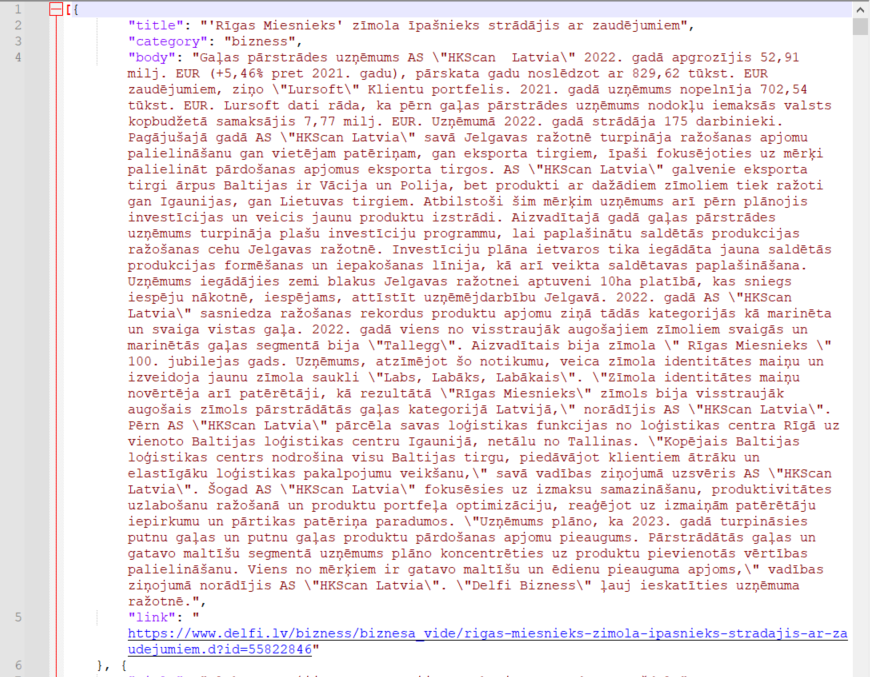
\includegraphics[width=\textwidth]{raksta_piemers}
\addtocounter{nofappendices}{1}
\label{appendix:raksta_piemers}

\section{Loģistiskās regresijas, KNT un LSTM modeļu salīdzinājums - Xiang Zhang}
\noindent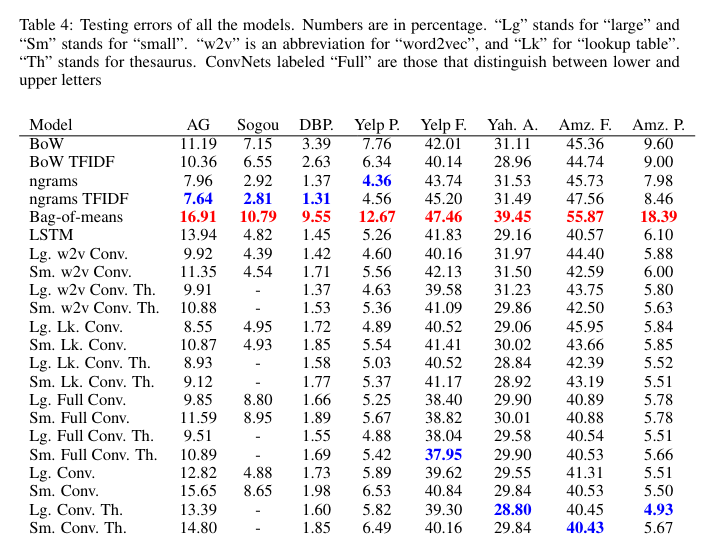
\includegraphics[width=\textwidth]{Model_Comp_Zhang}
\addtocounter{nofappendices}{1}
\label{appendix:zhang_models}

\section{Loģistiskās regresijas, KNT un LSTM modeļu salīdzinājums - Mathieu Cliche}
\noindent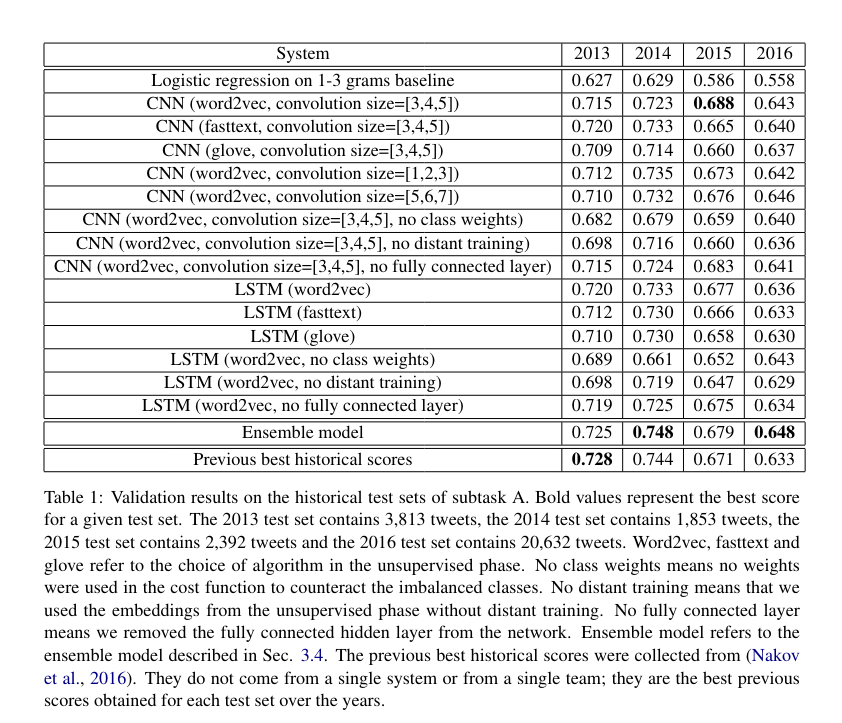
\includegraphics[width=\textwidth]{twitter_LSTM_CNN_comp}
\addtocounter{nofappendices}{1}
\label{appendix:twitter_models}

\section{Klasificējamo kategoriju rakstu garumi}
\noindent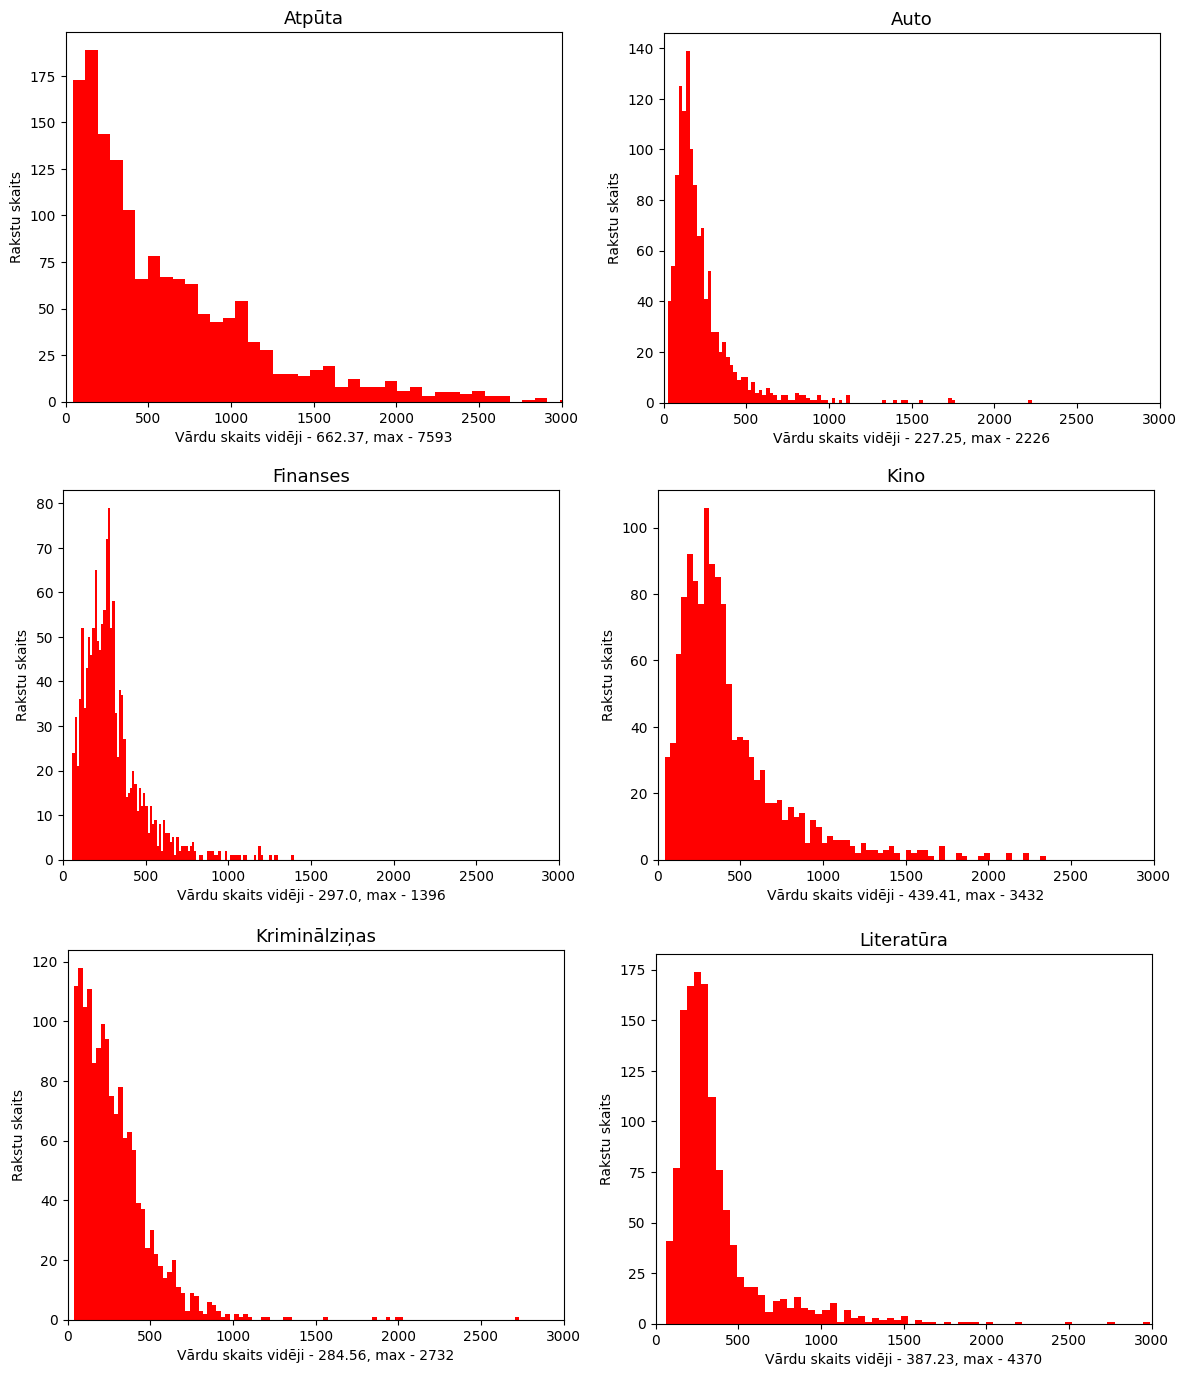
\includegraphics[width=\textwidth]{kategorijas_wc}
\noindent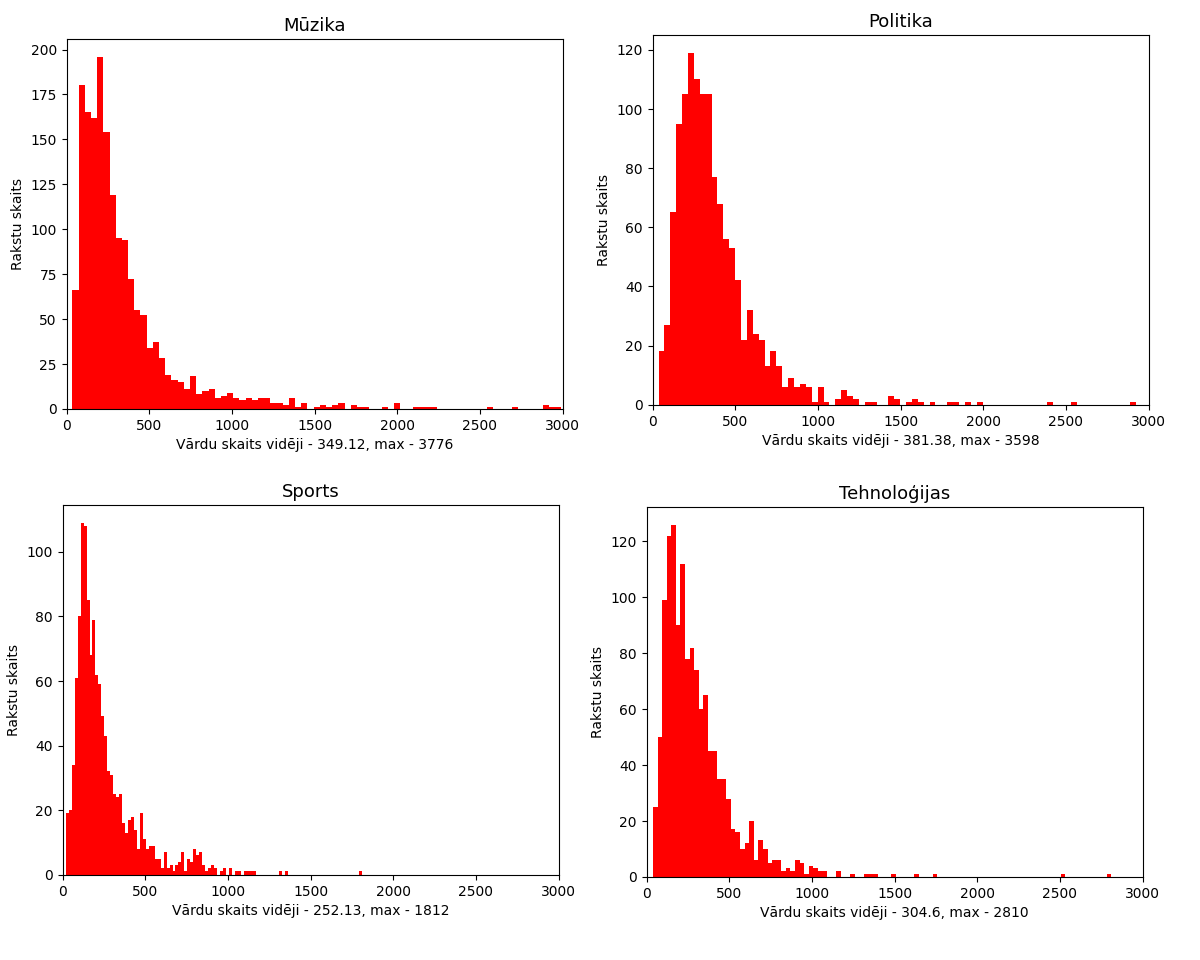
\includegraphics[width=\textwidth]{kategorijas_wc2}
\addtocounter{nofappendices}{1}
\label{appendix:kategorijas_wc}
